
\label{subsec:ANN:TDNN}

Prediction requires the use of dynamic neural networks, as discussed in
Chapter 14. The specific form of the network will depend on the particular
application. The simplest network for nonlinear prediction is the focused
time-delay neural network, which is shown in Figure 22.3. This is part of a
general class of dynamic networks, called focused networks, in which the
dynamics appear only at the input layer of a static multilayer feedforward
network. This network has the advantage that it can be trained using static
backpropagation algorithms, since the tapped-delay-line at the input of the
network can be replaced with an extended vector of delayed values of the
input.

\begin{figure}[!ht]
\centering
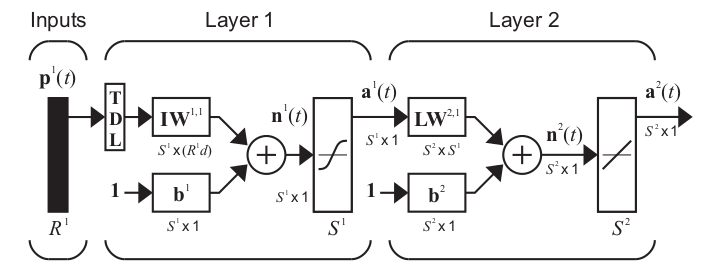
\includegraphics[width=\textwidth]{images/tdnn.png}
\caption{Time Delay network}
\label{fig:tdnn}
\end{figure}
